\subsection{Results}
	\begin{frame}{Small Domains}
		\resizebox{\linewidth}{!}{
			\centering
\begin{tabular}{| c | l | c | c | c | c | }
	\hline
	Dataset & Approach & Best Score & Avg. Initial Score & Avg. Best Score & Avg. It. \\ \hline
	\multirow{3}{*}{Census} & Random & \alert{-212186.79} & -213074.18 $\pm$ 558.43 & -212342.26 $\pm$ 174.21 & 7.26 $\pm$ 2.90 \\ \cline{2-6} 
			& DFS-based & -212190.05 & -212736.80 $\pm$ 379.96 & -212339.83 $\pm$ 152.26 & 5.90 $\pm$ 2.61 \\ \cline{2-6}
			& FAS-based & -212191.64 & \alert{-212287.99 $\pm$ 92.54} & \alert{-212222.12 $\pm$ 70.99} & \alert{3.28 $\pm$ 1.67} \\ \hline \hline

	\multirow{3}{*}{Letter} & Random & -138652.66 & -139774.54 $\pm$ 413.74 & -139107.13 $\pm$ 329.15 & 6.07 $\pm$ 2.50 \\ \cline{2-6} 
			& DFS-based & -138652.66 & -139521.38 $\pm$ 396.61 & \alert{-138999.84 $\pm$ 310.06} & 5.75 $\pm$ 2.35 \\ \cline{2-6}
			& FAS-based & -138652.66 & \alert{-139050.43 $\pm$ 70.55} & -139039.26 $\pm$ 87.97 & \alert{2.24 $\pm$ 0.96} \\ \hline \hline

	\multirow{3}{*}{Image} & Random & \alert{-12826.08} & -13017.13 $\pm$ 44.35 & -12924.24 $\pm$ 41.39 & 7.59 $\pm$ 2.71 \\ \cline{2-6} 
			& DFS-based & -12829.10 & -12999.09 $\pm$ 38.56 & -12921.13 $\pm$ 37.88 & 7.10 $\pm$ 2.47 \\ \cline{2-6}
			& FAS-based & -12829.10 & \alert{-12930.63 $\pm$ 20.83} & \alert{-12882.30 $\pm$ 26.43} & \alert{5.05 $\pm$ 1.72} \\ \hline \hline

	\multirow{3}{*}{Mushroom} & Random & \alert{-55513.38} & -58450.72 $\pm$ 1016.54 & -56563.84 $\pm$ 616.59 & 7.59 $\pm$ 2.76 \\ \cline{2-6} 
			& DFS-based & \alert{-55513.38} & -58367.11 $\pm$ 871.25 & -56472.72 $\pm$ 546.19 & 7.75 $\pm$ 2.58 \\ \cline{2-6}
			& FAS-based & -55574.71 & \alert{-56450.49 $\pm$ 154.54} & \alert{-56198.66 $\pm$ 174.64} & \alert{4.65 $\pm$ 1.63} \\ \hline \hline

	\multirow{3}{*}{Sensors} & Random & \alert{-62062.13} & -63476.33 $\pm$ 265.46 & -62726.60 $\pm$ 251.26 & 9.22 $\pm$ 2.94 \\ \cline{2-6} 
			& DFS-based & -62083.21 & -63392.60 $\pm$ 255.90 & -62711.50 $\pm$ 257.79 & 9.65 $\pm$ 3.12 \\ \cline{2-6}
			& FAS-based & -62074.88 & \alert{-62530.26 $\pm$ 133.44} & \alert{-62330.94 $\pm$ 121.82} & \alert{5.17 $\pm$ 2.24} \\ \hline
\end{tabular}
		}
	\end{frame}
	
	\begin{frame}{Large Domains}
		\resizebox{\linewidth}{!}{
			\begin{tabular}{| c | l | c | c | c | c | }
	\hline
	Dataset & Approach & Best Score & Avg. Initial Score & Avg. Best Score & Avg. It. \\ \hline
				
	\multirow{3}{*}{SteelPlates} & Random & -13336.14 & -13566.50 $\pm$ 65.80 & -13429.13 $\pm$ 52.14 & 8.96 $\pm$ 3.43 \\ \cline{2-6} 
			& DFS-based & \alert{-13332.91} & -13572.77 $\pm$ 81.12 & -13432.30 $\pm$ 57.57 & 9.30 $\pm$ 3.38 \\ \cline{2-6}
			& FAS-based & -13341.73 & \alert{-13485.26 $\pm$ 38.27} & \alert{-13397.08 $\pm$ 29.53} & \alert{7.77 $\pm$ 2.24} \\ \hline \hline
						
	\multirow{3}{*}{Epigenetics} & Random & -56873.76 & -57722.30 $\pm$ 228.44 & -57357.60 $\pm$ 222.12 & 5.89 $\pm$ 2.67 \\ \cline{2-6} 
			& DFS-based & \alert{-56868.87} & \alert{-57615.36 $\pm$ 189.17} & \alert{-57308.93 $\pm$ 165.18} & 6.42 $\pm$ 2.47 \\ \cline{2-6}
			& FAS-based & \alert{-56868.87} & -57660.09 $\pm$ 146.45 & -57379.59 $\pm$ 148.42 & \alert{5.33 $\pm$ 2.28} \\ \hline \hline

	\multirow{3}{*}{Alarm} & Random & -13218.22 & -13324.52 $\pm$ 30.49 & -13245.43 $\pm$ 15.63 & 10.92 $\pm$ 3.24 \\ \cline{2-6} 
			& DFS-based & \alert{-13217.97} & -13250.72 $\pm$ 17.70 & -13236.71 $\pm$ 12.02 & \alert{4.32 $\pm$ 2.32} \\ \cline{2-6}
			& FAS-based & -13220.55 & \alert{-13249.77 $\pm$ 2.57} & \alert{-13233.98 $\pm$ 6.19} & 6.34 $\pm$ 1.74 \\ \hline \hline

	\multirow{3}{*}{Spectf} & Random & -8176.81 & -8202.03 $\pm$ 5.23 & -8189.69 $\pm$ 4.65 & 7.20 $\pm$ 2.17 \\ \cline{2-6} 
			& DFS-based & \alert{-8172.37} & -8200.04 $\pm$ 4.08 & -8187.29 $\pm$ 4.91 & 7.86 $\pm$ 2.49 \\ \cline{2-6}
			& FAS-based & -8172.51 & \alert{-8176.98 $\pm$ 2.01} & \alert{-8176.07 $\pm$ 2.05} & \alert{2.27 $\pm$ 1.11} \\ \hline \hline 
					
	\multirow{3}{*}{LungCancer} & Random & \alert{-711.23} & -723.79 $\pm$ 2.69 & -718.03 $\pm$ 2.84 & 5.46 $\pm$ 1.78 \\ \cline{2-6} 
			& DFS-based & -711.36 & -720.47 $\pm$ 2.51 & \alert{-715.29 $\pm$ 1.86} & 5.02 $\pm$ 1.50 \\ \cline{2-6}
			& FAS-based & -711.39 & \alert{-716.13 $\pm$ 0.89} & -715.67 $\pm$ 1.19 & \alert{2.73 $\pm$ 1.79} \\ \hline
\end{tabular}
		}
	\end{frame}
	
	\begin{frame}
		\begin{columns}
			\begin{column}{.3\textwidth}
				\vskip-3em
				\begin{figure}
					\centering
					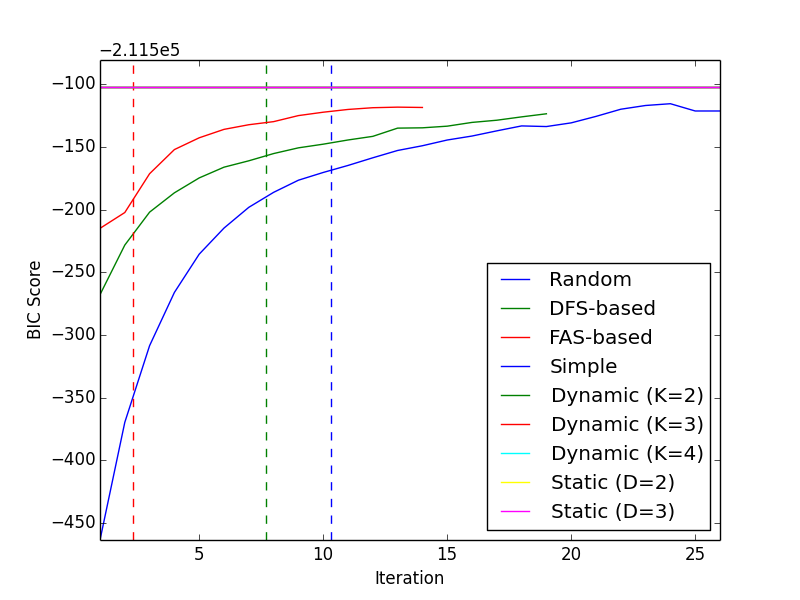
\includegraphics[height = 7em]{images/census}
					\caption{Census}
				\end{figure}
				\vskip-3em
				\begin{figure}
					\centering
					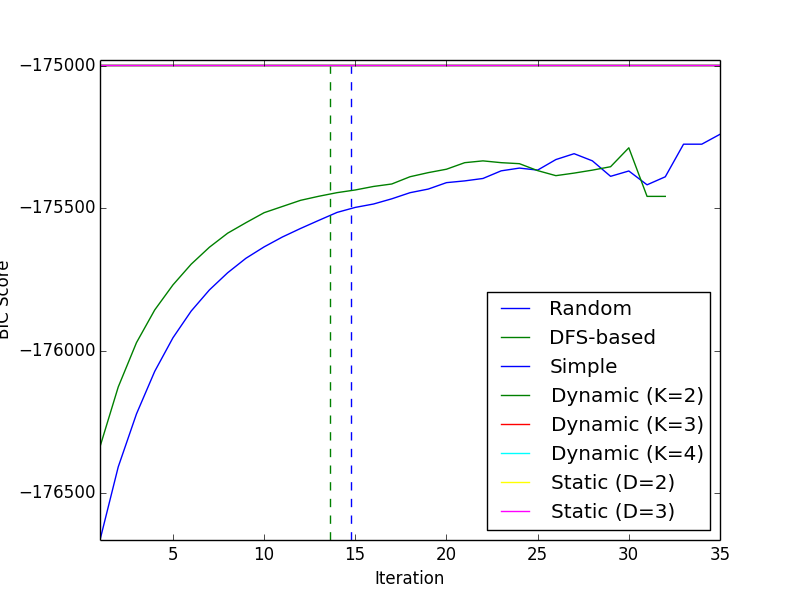
\includegraphics[height = 7em]{images/letter}
					\caption{Letter}
				\end{figure}
			\end{column}
			\begin{column}{.3\textwidth}
				\begin{figure}
					\centering
					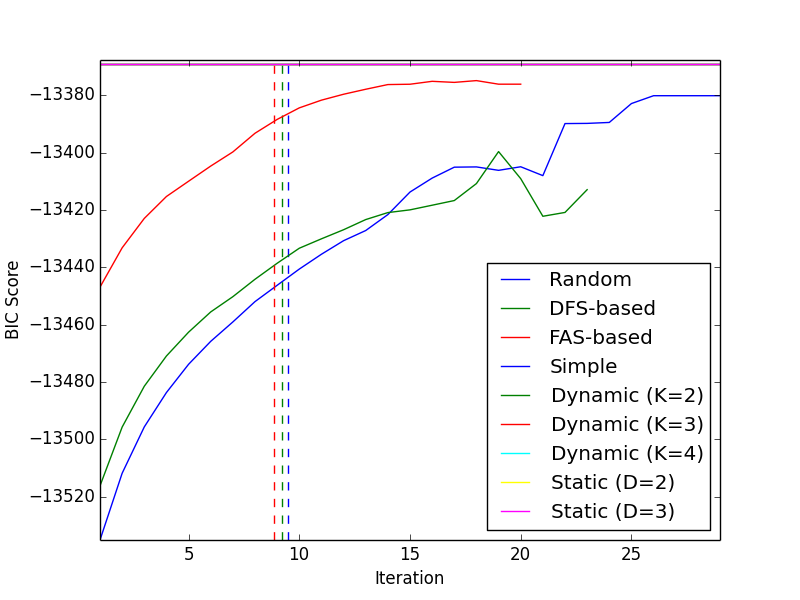
\includegraphics[height = 7em]{images/image}
					\caption{Image}
				\end{figure}
			\end{column}
			\begin{column}{.3\textwidth}
				\vskip-3em
				\begin{figure}
					\centering
					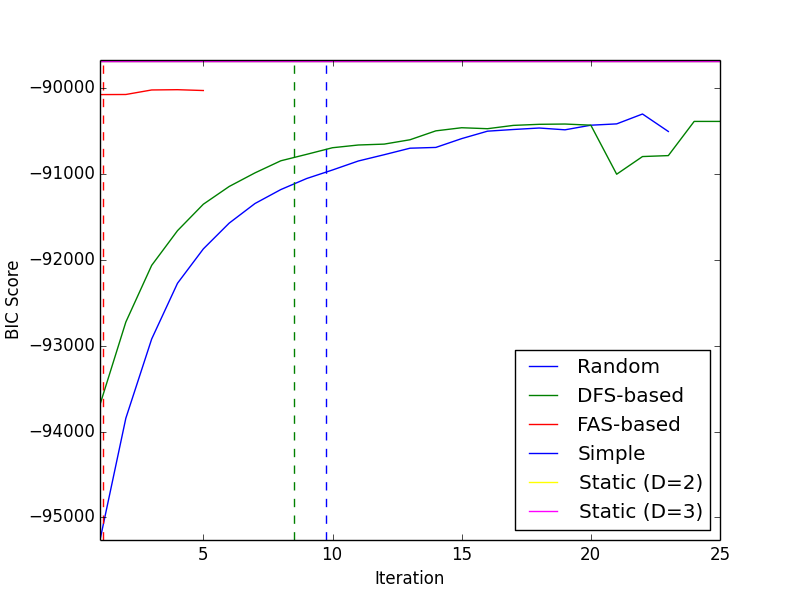
\includegraphics[height = 7em]{images/mushroom}
					\caption{Mushroom}
				\end{figure}
				\vskip-3em
				\begin{figure}
					\centering
					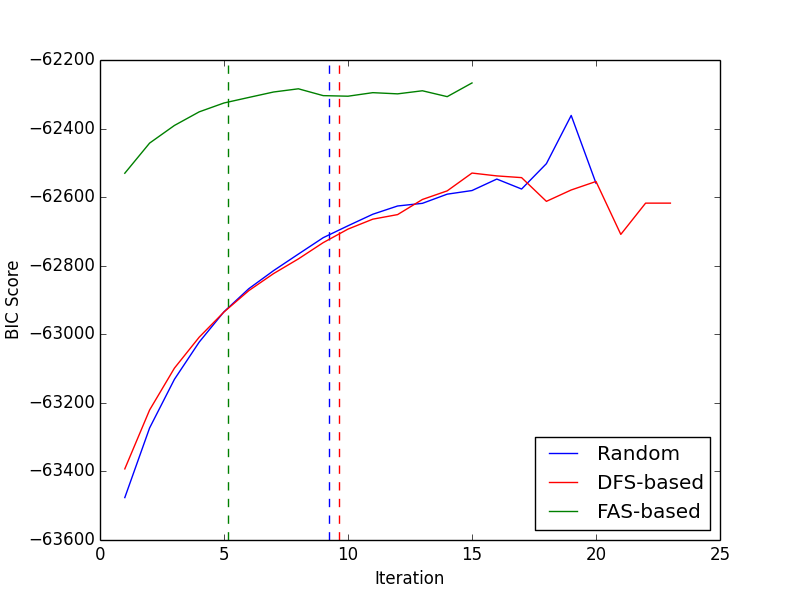
\includegraphics[height = 7em]{images/sensors}
					\caption{Sensors}
				\end{figure}
			\end{column}
		\end{columns}
	\end{frame}

	
	\begin{frame}
		\begin{columns}
			\begin{column}{.3\textwidth}
				\vskip-3em
				\begin{figure}
					\centering
					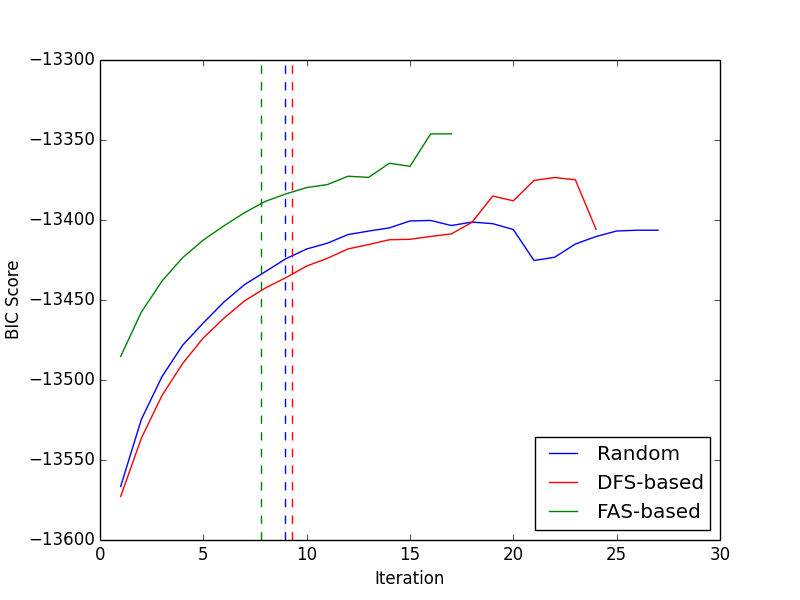
\includegraphics[height = 7em]{images/steelPlates}
					\caption{SteelPlates}
				\end{figure}
				\vskip-3em
				\begin{figure}
					\centering
					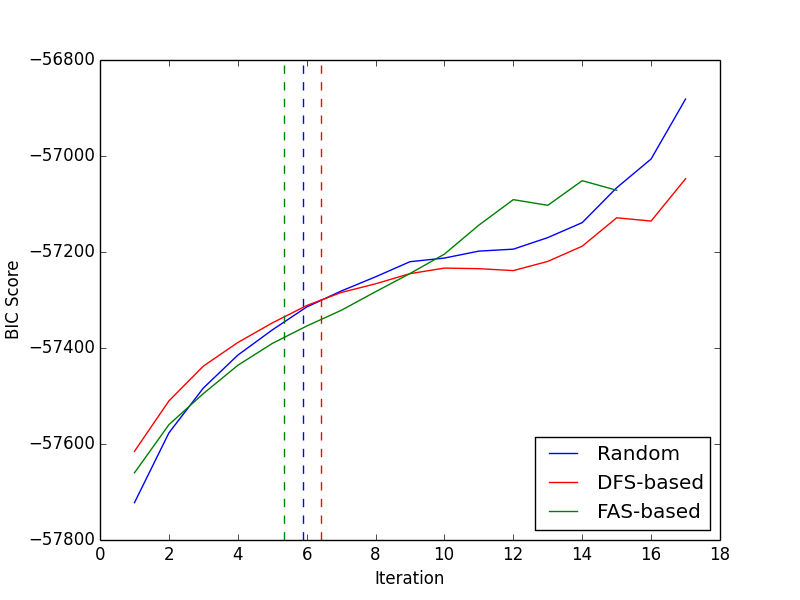
\includegraphics[height = 7em]{images/epigenetics}
					\caption{Epigenetics}
				\end{figure}
			\end{column}
			\begin{column}{.3\textwidth}
				\begin{figure}
					\centering
					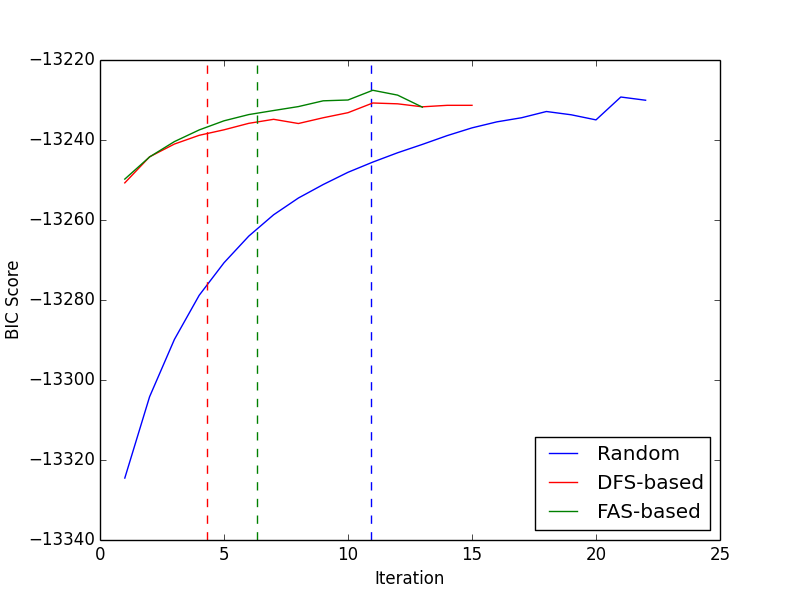
\includegraphics[height = 7em]{images/alarm}
					\caption{Alarm}
				\end{figure}
			\end{column}
			\begin{column}{.3\textwidth}
				\vskip-3em
				\begin{figure}
					\centering
					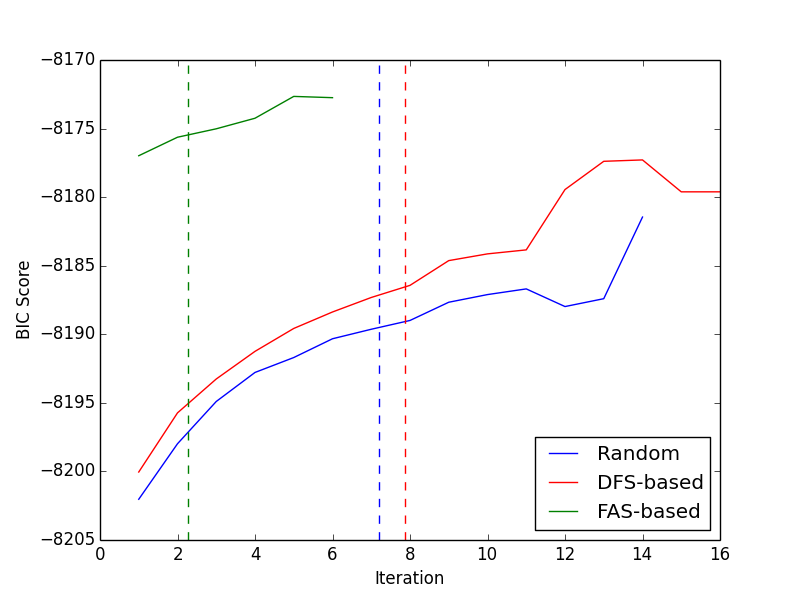
\includegraphics[height = 7em]{images/spectf}
					\caption{Spectf}
				\end{figure}
				\vskip-3em
				\begin{figure}
					\centering
					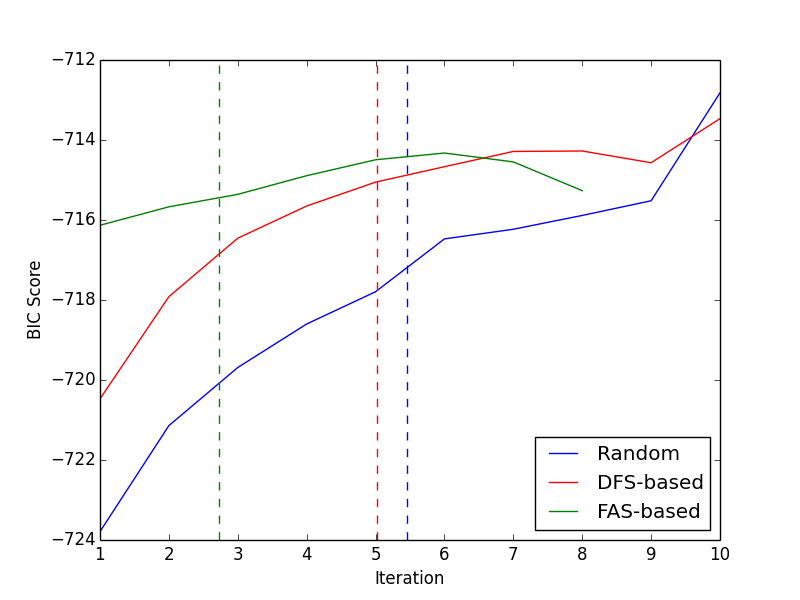
\includegraphics[height = 7em]{images/lungCancer}
					\caption{LungCanc}
				\end{figure}
			\end{column}
		\end{columns}
	\end{frame}